\chapter{Results}
\label{chap:results}

In this chapter, the results of evaluating the TinyFuncCoder series on the various metrics introduced in section \ref{sec:metrics} will be presented in section \ref{sec:metricresults}, with an overview of the total results in section \ref{sec:resoverview}.
Further, results of the exploratory training tests of section \ref{sec:pretrain} are given in section \ref{sec:pretrainres} and the loss progression during training is given in section \ref{sec:loss}.

\section{Exploratory Training Results}
\label{sec:pretrainres}
This section will present the results of the exploratory training done in section \ref{sec:pretrain}.
These models are only evaluated on HumanEval and HumanEval+ as a starting point, to see which training methods are viable.
Later, the TinyFuncCoder models will be evaluated on a bigger test suite.
Testing the initial batch of models trained on 1\% of the dataset (fixed and stratified) on HumanEval resulted in a pass@1 of under 10\% for each model, with the best performing reaching 9.1\% and the worst 2.4\%.
HumanEval+ reduced these to 6.7\% and 1.8\% respectively.
Important to note is that during generation of the worst results, the start token was not appended to the start of the problem, strongly strengthening the assumption that tokens are important for the model.
Calculating pass@10 for the best model results in minor improvements, with HumanEval rising to 9.8\% from 9.1\% and HumanEval+ rising to 7.9\% from 6.9\%. Fine-tuning models for multiple epochs seems to have no further learning effect when using the 1\% datasets.
The full results for the first batch of seeded training can be seen in figure \ref{fig:pretrainone}.
As can be seen, the results hover around the same percentage ranges of around 7-10\% for HumanEval and 6-8\% for HumanEval+, with the main outlier being the model that did not use start and end tokens for the functions.
This shows the importance of the tokens, but also that all chosen chunks of data seem to provide a similar learning effect.
Further fine-tuning on the same data also seems to have little to no effect on performance, decreasing it if anything.
It is also notable that the best performing model was the one trained on two seperate chunks of data.
This, combined with the fact that same-chunk multi-episode tuning did not improve, inspired the experiments with multi-chunk training to come.

\begin{figure}[H]
    \centering
    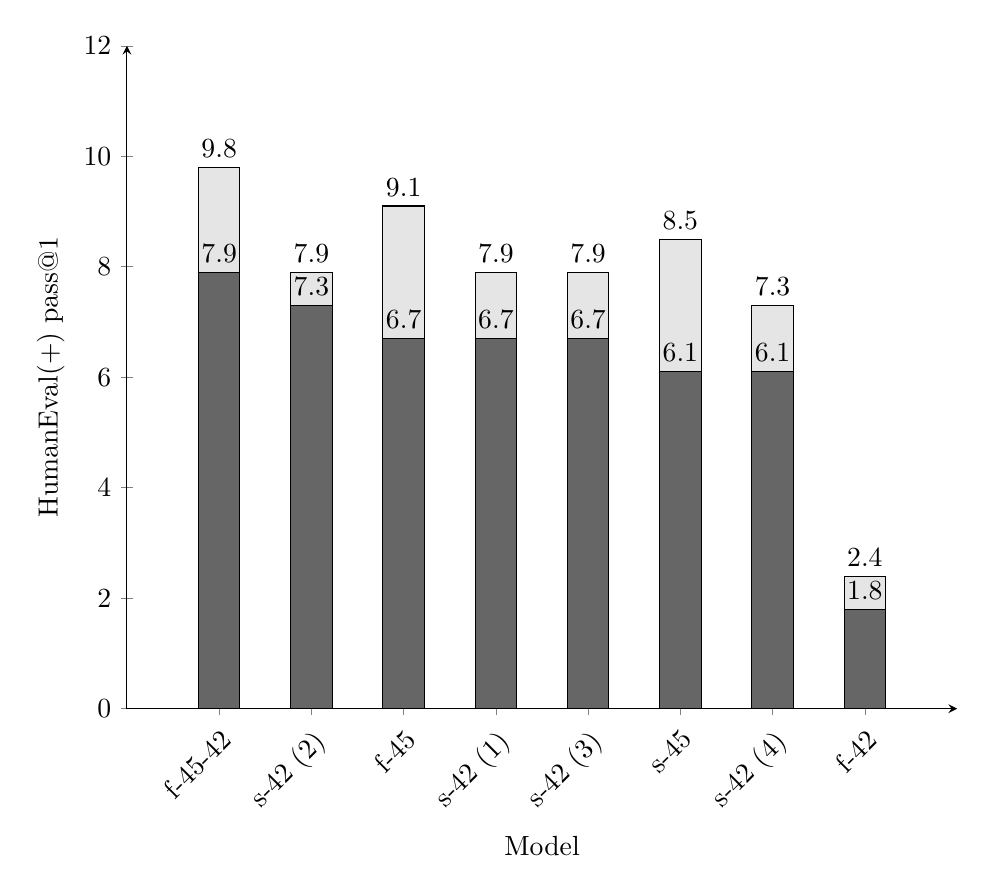
\begin{tikzpicture}
        \begin{axis}[
            ybar,
            xtick={0,1,2,3,4,5,6,7},
            xticklabels={f-45-42, s-42 (2), f-45, s-42 (1), s-42 (3), s-45, s-42 (4), f-42},
            ylabel={HumanEval(+) pass@1},
            xlabel={Model},
            ymin=0,
            ymax=12,
            bar width=15pt,
            nodes near coords,
            width=\textwidth,
            height=10cm,
            enlarge x limits=0.15,
            x tick label style={rotate=45, anchor=north east},
            axis x line=bottom,
            axis y line=left,
            every axis plot/.append style={bar shift=0pt},
            xmin=-1,
            xmax=8
        ]
    
        % HumanEval
        \addplot[ybar,fill=black!10] plot coordinates {(0, 9.8) (1, 7.9) (2, 9.1) (3, 7.9) (4, 7.9) (5, 8.5) (6, 7.3) (7, 2.4)};
    
        % HumanEval+
        \addplot[ybar,fill=black!60] plot coordinates {(0, 7.9) (1, 7.3) (2, 6.7) (3, 6.7) (4, 6.7) (5, 6.1) (6, 6.1) (7, 1.8)};
    
        \end{axis}
    \end{tikzpicture}
    \caption{Pass@1 rates for HumanEval (light bar) and HumanEval+ (dark bar) with TinyLlama-v1.0 fine-tuned on various dataset samples. f and s refer to stratified and fixed sampling, the number after the dash to the seed used for sampling. The number in the brackets refers to the epoch count, if it was trained for multiple (on the same dataset). f-42 did not use the start and end tokens. f-45-42 was trained on the fixed-45 sample, then the fixed-42 sample (with tokens).}
    \label{fig:pretrainone}
\end{figure}

The second round of testing was to see if altering the \ac{lora} rank and alpha values could improve performance.
Starting here, fine-tuning was done with stratified sampled chunks with seeds counting up from 0.
In this case, where only one episode was trained, the data was seeded with 0.
The combinations tested were the original rank 64 alpha 16 as well as two adaptations for the double and half rule: rank 64 alpha 32 and rank 8 alpha 16.
As can be seen in figure \ref{fig:pretraintwo}, the other variants performed worse than the original.

\begin{figure}[H]
    \centering
    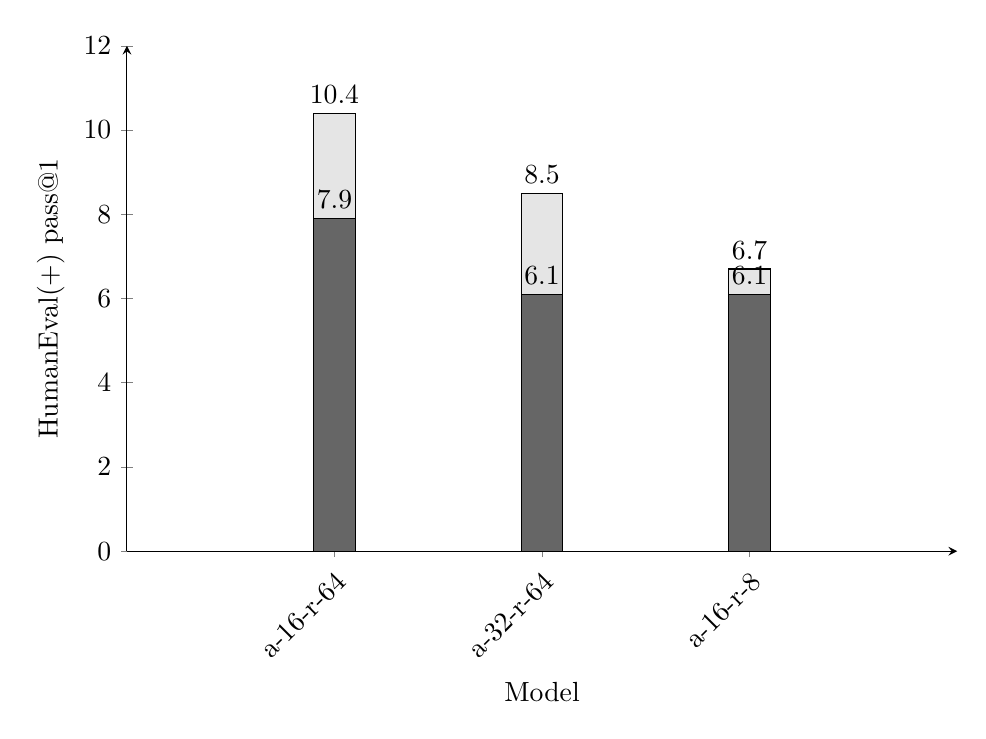
\begin{tikzpicture}
        \begin{axis}[
            ybar,
            xtick={0,1,2},
            xticklabels={a-16-r-64, a-32-r-64, a-16-r-8},
            ylabel={HumanEval(+) pass@1},
            xlabel={Model},
            ymin=0,
            ymax=12,
            bar width=15pt,
            nodes near coords,
            width=\textwidth,
            height=8cm,
            enlarge x limits=0.15,
            x tick label style={rotate=45, anchor=north east},
            axis x line=bottom,
            axis y line=left,
            every axis plot/.append style={bar shift=0pt},
            xmin=-1,
            xmax=3
        ]

        % HumanEval
        \addplot[ybar,fill=black!10] plot coordinates {(2, 6.7) (0, 10.4) (1, 8.5)};

        % HumanEval+
        \addplot[ybar,fill=black!60] plot coordinates {(2, 6.1) (0, 7.9) (1, 6.1)};

        \end{axis}
    \end{tikzpicture}
    \caption{Pass@1 rates for HumanEval (light bar) and HumanEval+ (dark bar) with TinyLlama-v1.0 fine-tuned on the first data chunk. a and r refer to alpha and rank, the number after the dash to their value.}
    \label{fig:pretraintwo}
\end{figure}

The final step of pre-testing was the experimentation for swapping out datasets mid-training.
The third iteration is not shown as it was visibly faulty when starting training and never finished an epoch, while the fourth iteration led into final training, the results of which are presented in the upcoming sections.
As seen in \ref{fig:pretrainthree}, the results are still concentrated around the same percentage values, while not necessarily improving with multiple epochs.
Also notable is that the HumanEval and HumanEval+ results improved over the results from the same configuration in figure \ref{fig:pretraintwo} (a-16-r-64 and v1 (1) are trained identically).
This is due to the temperature of the generator pipeline, resulting in slight variations in score when generating.
The temperature is taken from the model, in this case 1.0.
This is a discrepancy that was not noticed until final training began.
As there are no major outliers in evaluation so far, it can be assumed that this had no major impact on the results for final training.

Because results did not improve with training, and because using seeded sampling could still cause overlap in data trained on, leading to unpredictable training data and results, the data was split into 100 stratified chunks that were saved locally.
These chunks contain no overlap, instead being an even division of the data.
This, along with the other changes of the fourth iteration, were hoped to result in better performance when training for more epochs.

\begin{figure}[H]
    \centering
    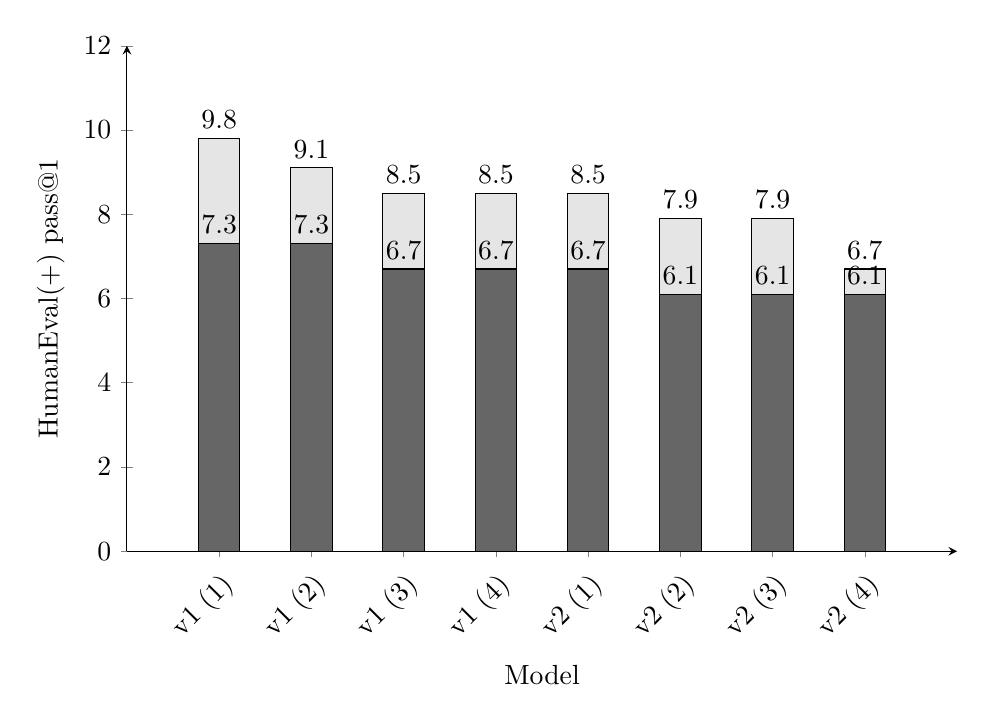
\begin{tikzpicture}
        \begin{axis}[
            ybar,
            xtick={0,1,2,3,4,5,6,7},
            xticklabels={v1 (1), v1 (2), v1 (3), v1 (4), v2 (1), v2 (2), v2 (3), v2 (4)},
            ylabel={HumanEval(+) pass@1},
            xlabel={Model},
            ymin=0,
            ymax=12,
            bar width=15pt,
            nodes near coords,
            width=\textwidth,
            height=8cm,
            enlarge x limits=0.15,
            x tick label style={rotate=45, anchor=north east},
            axis x line=bottom,
            axis y line=left,
            every axis plot/.append style={bar shift=0pt},
            xmin=-1,
            xmax=8
        ]

        % HumanEval
        \addplot[ybar,fill=black!10] plot coordinates {(7, 6.7) (5, 7.9) (1, 9.1)(2, 8.5) (0,9.8) (6,7.9) (3, 8.5) (4,8.5)};

        % HumanEval+
        \addplot[ybar,fill=black!60] plot coordinates {(7, 6.1) (5, 6.1) (1, 7.3)(2, 6.7) (0,7.3) (6,6.1) (3,6.7) (4,6.7)};

        \end{axis}
    \end{tikzpicture}
    \caption{Pass@1 rates for HumanEval (light bar) and HumanEval+ (dark bar) with TinyLlama-v1.0 fine-tuned on various dataset samples. v1 and v2 refer to the first and second iteration described in section \ref{sec:pretrain}, the bracketed number to the epoch count. As seeds count up from 0, epoch 4 is trained on data from seeds 0, 1, 2 and 3.}
    \label{fig:pretrainthree}
\end{figure}


\section{Results on Code Synthesis Metrics}
\label{sec:metricresults}

This section will show the results on all chosen metrics individually, with an overview of all results in section \ref{sec:resoverview}.
In this section, the TinyLlama models will be abbreviated as TL and the TinyFuncCoder models as TFC.
Reformatted prompts (R) indicate prompts that have been altered to fit TinyFuncCoder's data scheme from training, namely <func>, the language as a comment, the docstring, then the head and parameters.
Any extra information such as imports or class structures is put before the function tag.

\subsection{Results Overview}
\label{sec:resoverview}
This section will provide an overview of the main results, compiling all individual metrics into a single table.
For metrics that are divided into multiple categories, like DS-1000, the average of all categories is given.
Each metric is discussed individually in the upcoming sections.

\begin{table}[h]
    \centering
    \small
    \caption{Pass@1 comparison between the TinyFuncCoder series and TinyLlama series on all metrics. TinyLlama values were calculated alongside TinyFunc-
    Coder. (R) indicates a reformatted prompt for evaluation. For the multi-value metrics, DS-1000, MultiPL-E and HumanEvalPack, the average was taken. HumanEvalPack was not included as it is equivalent to HumanEval, as discussed in section \ref{sec:humanevalpackres}.}
    \begin{tabular}{l|rrrrrr}
        \hline
        Model & Human & MBPP(+) & MultiPL-E & MultiPL-E & DS-1000 & Avg. \\
         & Eval(+) & & (featured) & (other) & \\
        \hline
        TL-v1.0 & 12.20 (10.98) & 0.60 (0.53) & 3.76 & 6.64 & 1.60 & 5.19 \\
        \textbf{TFC-v1.0} & \textbf{9.76 (8.54)} & \textbf{8.20 (9.26)} & \textbf{7.52} & \textbf{8.68} & \textbf{0.70} & \textbf{7.45} \\
        TL-v1.1 & 1.22 (1.22) & 2.60 (3.17) & 2.46 & 6.57 & 0.70 & 2.56 \\
        TL-v1.1\_mc & 6.70 (4.88) & 13.00 (17.20) & 5.55 & 9.08 & 1.80 & 8.32 \\
        \textbf{TFC-v1.1} & \textbf{0.00 (0.00)} & \textbf{0.00 (0.00)} & \textbf{0.00} & \textbf{0.00} & \textbf{0.00} & \textbf{0.00} \\
        \hline
        TL-v1.0 (R) & 7.93 (7.32) & 12.00 (15.08) & 4.46 & - & 0.10 & 7.82 \\
        \textbf{TFC-v1.0 (R)} & \textbf{9.76 (8.54)} & \textbf{12.80 (19.58)} & \textbf{11.07} & \textbf{-} & \textbf{1.00} & \textbf{10.46} \\
        TL-v1.1 (R) & 3.66 (3.66) & 3.00 (4.50) & 2.82 & - & 0.20 & 2.97 \\
        TL-v1.1\_mc (R) & 14.02 (12.20) & 8.20 (10.85) & 6.89 & - & 0.10 & 8.71 \\
        \textbf{TFC-v1.1 (R)} & \textbf{0.00 (0.00)} & \textbf{0.00 (0.26)} & \textbf{0.00} & \textbf{-} & \textbf{0.00} & \textbf{0.04} \\
        \hline
    \end{tabular}
    \label{tab:resoverview}
\end{table}

As can be seen in table \ref{tab:resoverview}, TinyFuncCoder-v1.0 improves over TinyLlama-v1.0 in some metrics while worsening in others, and TinyFuncCoder-v1.1 is broadly unsuccessful in generating correct solutions.
The TinyFuncCoder-v1.0 average sits above TinyLlama-v1.0, and even above TinyLlama-v1.1\_math\_code when taking the reformatted prompt into consideration.
However, this is likely inflated due to PHP and Go, as will be discussed in section \ref{sec:multipleres}.


\subsection{Results on HumanEval(+)}
\label{sec:humanevalres}

This section will showcase TinyFuncCoder performance on HumanEval.
Because this is the most well-known and commonly used evaluation metric for code synthesis models, it was also used for evaluating TinyFuncCoder-v1.0 after each training epoch to see if model improvements could be monitored.
The results to this are shown in figure \ref{fig:humaneval}.
% TODO reevaluate with merging PEFT model & proper temperature! (at TransforMA/human-eval/results/chunked/...)
\begin{figure}[!h]
    \centering
    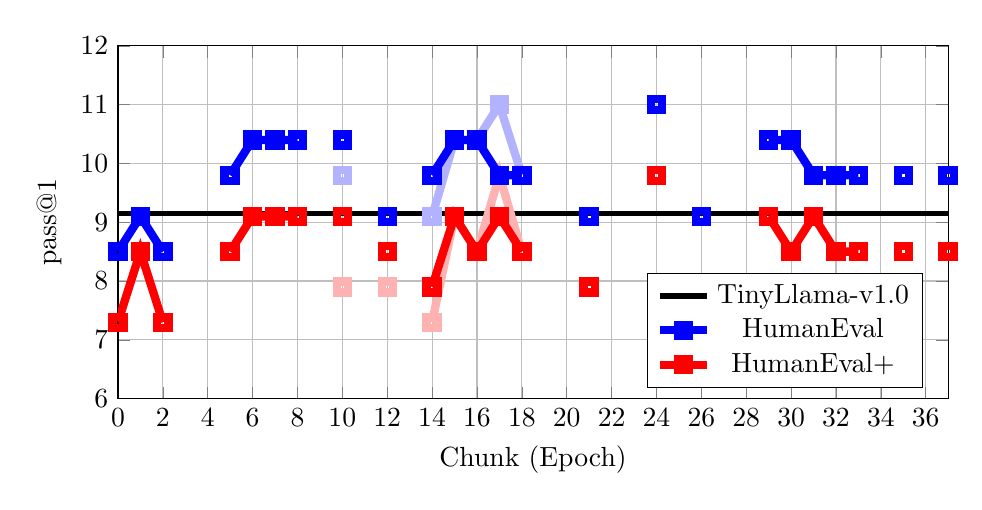
\begin{tikzpicture}
        \begin{axis}[
            xlabel={Chunk (Epoch)},
            ylabel={pass@1},
            ymin=6,
            ymax=12,
            xmin=0,
            xmax=37,
            xtick distance=2,
            ytick distance=1,
            grid=major,
            width=\textwidth,
            height=\textwidth/2,
            legend pos=south east,
            every axis plot/.append style={thick, line width=3pt},
        ]
        
        \addlegendimage{black, thick, line width=2pt}
        \addlegendentry{TinyLlama-v1.0}
        
        \addlegendimage{blue, thick, mark=square, line width=3pt}
        \addlegendentry{HumanEval}

        \addlegendimage{red, thick, mark=square, line width=3pt}
        \addlegendentry{HumanEval+}

        \addplot[
            color=black,
            thick,
            domain=0:37,
            line width=2pt
        ]
        {9.15};
        
        %%%%%%%%%%%%%%%%%%%%%%%%%%%%%%%%%%%%%%%%%%%%%%%%%%%%%%%%%
        \addplot[color=blue!30,mark=square]
        coordinates {
            (10,9.8)
            
            (12,9.1)
            
            (14,9.1) (15,10.4) (16,10.4) (17,11) (18,9.8)
        };
        %%%%%%%%%%%%%%%%%%%%%%%%%%%%%%%%%%%%%%%%%%%%%%%%%%%%%%%%%
        \addplot[color=red!30,mark=square]
        coordinates {
            (10,7.9)
            
            (12,7.9)
            
            (14,7.3) (15,9.1) (16,8.5) (17,9.8) (18,8.5)
        };
        %%%%%%%%%%%%%%%%%%%%%%%%%%%%%%%%%%%%%%%%%%%%%%%%%%%%%%%%%
        \addplot[color=blue!100,mark=square]
        coordinates {
            (0,8.5) (1,9.1) (2,8.5)
        
            (5,9.8) (6,10.4) (7,10.4) (8,10.4)
            
            (10,10.4)
            
            (12,9.1)
            
            (14,9.8) (15,10.4) (16,10.4) (17,9.8) (18,9.8)
            
            (21,9.1)
            
            (24,11)
            
            (26,9.1)
            
            (29,10.4) (30,10.4) (31,9.8) (32,9.8) (33,9.8)
            
            (35,9.8)
            
            (37,9.8)
        };
        %%%%%%%%%%%%%%%%%%%%%%%%%%%%%%%%%%%%%%%%%%%%%%%%%%%%%%%%%
        \addplot[color=red!100,mark=square]
        coordinates {
            (0,7.3) (1,8.5) (2,7.3)
            
            (5,8.5) (6,9.1) (7,9.1) (8,9.1)
            
            (10,9.1)
            
            (12,8.5)
            
            (14,7.9) (15,9.1) (16,8.5) (17,9.1) (18,8.5)
            
            (21,7.9)
            
            (24,9.8)
            
            (26,7.9)
            
            (29,9.1) (30,8.5) (31,9.1) (32,8.5) (33,8.5)
            
            (35,8.5)
            
            (37,8.5)
        };
        %%%%%%%%%%%%%%%%%%%%%%%%%%%%%%%%%%%%%%%%%%%%%%%%%%%%%%%%%
        \end{axis}
    \end{tikzpicture}
    \caption{Pass@1 on HumanEval and HumanEval+ for each epoch TinyLlama-v1.0 was fine-tuned. Chunks without a point have been skipped due to memory crashes. The black line shows TinyLlama's performance on HumanEval without any fine-tuning.
    The lighter lines are performance of the checkpoints trained from the wrong starting point, as mentioned in section \ref{sec:finaltrain}. If the blue line goes below the black, the model's performance has worsened from fine-tuning. Model performance was evaluated with the EvalPlus implementation, not the Bigcode Evaluation Harness implementation.}
    \label{fig:humaneval}
\end{figure}

While model performance on HumanEval(+) is unstable, the tendancy does trend upwards. The earliest epochs perform worse than the base model, but improve to be equal to or better than TinyLlama-v1.0 after just a few epochs.
It can also be noted that HumanEval and HumanEval+ performance is not directly linked.
For example, at chunk 17 HumanEval performance drops, but HumanEval+ performance rises.
This makes sense -- HumanEval+ expands the test suite for HumanEval.
A generation that HumanEval judged as correct could be rejected by HumanEval+, improving the former while keeping the latter the same.
Conversely, a task that was already correct according to HumanEval could be improved to also be approved by HumanEval+, keeping the former the same while improving the latter.
Also of note is that the training from a wrong starting checkpoint, shown in the lighter lines, match the best epoch of evaluation, 24.
Another important factor is the temperature used for generating.
For all results in this section, it is set to 0.2.
While this relatively low, it will still lead to some variance when generating answers.
Even when prompting an identical model multiple times with the same question, results may differ.
Performance can only improve or worsen in steps of $1/164$, or about 0.6\%, so correctly or incorrectly generating one or two questions due to variations caused by the temperature can already shift pass@1 by a percentage point.
Also interesting is that there are two sections where performance stays broadly consistens -- chunks six to ten and chunks 31 to 37.


\begin{table}[!h]
    \centering
    \caption{HumanEval(+) pass@1 comparison between the TinyFuncCoder series and contemporary models. Values taken from the EvalPlus leaderboard. Models without a size are closed-source. TinyLlama values were calculated alongside TinyFuncCoder. (R) indicates a reformatted prompt for evaluation.}
    \begin{tabular}{l|rr|r}
        \hline
        Model & HumanEval & HumanEval+ & Size \\
        \hline
        GPT-4-Turbo (April 2024) & 90.20 & 86.60 & - \\ claude-3-opus (Mar 2024) & 82.90 & 77.40 & - \\
        \hline
        DeepSeek-Coder-V2-Instruct & 88.40 & 82.30 & 236 B \\
        OpenCodeInterpreter-DS-33B & 79.30 & 73.80 & 33 B \\
        WizardCoder-33B-V1.1 & 79.90 & 73.20 & 33 B \\
        Magicoder-S-DS-6.7B & 76.80 & 71.30 & 6.7 B \\
        DeepSeek-Coder-1.3B-Base & 28.70 & 25.60 & 1.3 B \\
        \hline
        TL-v1.0 & 12.20 & 10.98 & 1.1 B \\
        \textbf{TFC-v1.0} & \textbf{9.76} & \textbf{8.54} & \textbf{1.1 B} \\
        TL-v1.1 & 1.22 & 1.22 & 1.1 B \\
        TL-v1.1\_mc & 6.70 & 4.88 & 1.1 B \\
        \textbf{TFC-v1.1 (R)} & \textbf{0.00} & \textbf{0.00} & \textbf{1.1 B} \\
        \hline
        TL-v1.0 (R) & 7.93 & 7.32 & 1.1 B \\
        \textbf{TFC-v1.0 (R)} & \textbf{9.76} & \textbf{8.54} & \textbf{1.1 B} \\
        TL-v1.1 (R) & 3.66 & 3.66 & 1.1 B \\
        TL-v1.1\_mc (R) & 14.02 & 12.20 & 1.1 B \\
        \textbf{TFC-v1.1 (R)} & \textbf{0.00} & \textbf{0.00} & \textbf{1.1 B} \\
        \hline
    \end{tabular}
    \label{tab:humaneval}
\end{table}

Table \ref{tab:humaneval} shows the pass@1 rates of TinyFuncCoder in comparison to other models presented in this thesis.
The rates of the other models come from the EvalPlus leaderboard\footnote{\url{https://evalplus.github.io/leaderboard.html} (last visited on 2024-10-31)}.
A few things become quickly apparent: pass@k rates seem to be proportional to model size, with bigger models having massively better results than smaller models.
This trend continues to the closed-source models as well -- GPT4 has been estimated to have 1.8 T parameters by multiple experts\footnote{\url{https://www.youtube.com/watch?v=K5iDUZPx60E&t=2989s} (last visited on 2024-10-31),
\\\url{https://www.semianalysis.com/p/gpt-4-architecture-infrastructure} (last visited on 2024-10-31),
\\\url{https://preview.redd.it/d-same-param-count-for-gpt4-from-nvidia-gtc24-as-the-leak-v0-vyzfx2sel5pc1.png?width=1764&format=png&auto=webp&s=58b33f4fe36915163f74ff9dea329af58be3ce51} (last visited on 2024-10-31),
\\\url{https://x.com/soumithchintala/status/1671267150101721090} (last visited on 2024-10-31)}.
As for the TinyLlama and the TinyFuncCoder series, the following is of note:
First, TinyFuncCoder-v1.0 is worse than its respective base model, and TinyFuncCoder-v1.1 has a pass rate of zero.
TinyLlama-v1.0 actually performs better than listed in their paper, scoring 12.2 rather than the 9.15 listed.
TinyFuncCoder-v1.0 does improve on the 9.15 listed, scoring 9.76 which is equivalent to one extra problem solved correctly, but not on the newly calculated 12.2.
It is also notable that reformatting the prompt to the TinyFuncCoder template has inconsistent effects among the models, with some improving (even drastically, like TinyLlama-v1.1\_math\_code, which more than doubles its pass@1), some becoming worse (like TinyLlama-v1.0), and TinyFuncCoder-v1.0 not being affected at all.
Surprisingly, even TinyLlama-v1.1 can generate some correct code without being explicitly trained on code, which makes the fact that TinyFuncCoder-v1.1 cannot even more surprising.
Overall, TinyFuncCoder does not improve on TinyLlama.
Further, DeepSeekCoder-1.3B-Base achieves between double and triple the performance with only an extra 200 M parameters.


\subsection{Results on MBPP(+)}
\label{sec:mbppres}

On MBPP(+), overall results -- shown in table \ref{tab:mbpp} -- are very similar to HumanEval, with increasing model size broadly translating to better performance.
DeepSeek-Coder-1.3B-Base also outperforms the TinyLlama and TinyFuncCoder models by a wide margin and TinyFuncCoder-v1.1 sits at zero again.
There are some unexpected results for this metric, starting with TinyLlama-v1.0, which performs surprisingly bad, even worse than v1.1 without code training.
Results were generated multiple times with unchanged performance.
Using the reformatted prompt, TinyLlama-v1.0 suddenly performs normally.
It is unclear what causes this behaviour.
Notably, TinyFuncCoder-v1.0 outperforms TinyLlama-v1.0 with a reformatted prompt, and is even comparable to TinyLlama-v1.1\_math\_code.
Next, performance on MBPP+ improves for the models evaluated for this thesis (TinyLlama and TinyFuncCoder), but worsens on all others.
This may be related to the fact that MBPP+ has 378 questions, while MBPP has 500.
$378/500$ gives a ratio of around 1.32 which is broadly consistent with the difference in MBPP to MBPP+ scores of the manually evaluated models (avg. 1.27, med. 1.29), but does not explain why the other models do not also experience this improvement.
MBPP+ also marks the only time where TinyFuncCoder-v1.1 generates a correct solution to any question in any metric.
Because of this, all discussions of TinyFuncCoders performance in upcoming chapters will focus on v1.0.
In summary, the best TinyFuncCoder results improve over the best TinyLlama results on MBPP and MBPP+.

\begin{table}[!h]
    \centering
    \caption{MBPP(+) pass@1 comparison between the TinyFuncCoder series and contemporary models. Values taken from the EvalPlus leaderboard. Models without a size are closed-source. TinyLlama values were calculated alongside TinyFuncCoder. (R) indicates a reformatted prompt for evaluation.}
    \begin{tabular}{l|rr|r}
        \hline
        Model & MBPP & MBPP+ & Size \\
        \hline
        claude-3-opus (Mar 2024) & 89.4 & 73.3 & - \\
        GPT-4-Turbo (Nov 2023) & 85.7 & 73.3 & - \\
        \hline
        DeepSeek-Coder-V2-Instruct & 89.40 & 75.10 & 236 B \\
        WizardCoder-Python-34B-V1.0 & 75.10 & 63.20 & 34 B \\
        OpenCodeInterpreter-DS-33B & 80.2 & 68.5 & 33 B \\
        Magicoder-S-DS-6.7B & 79.40 & 69.00 & 6.7 B \\
        DeepSeek-Coder-1.3B-Base & 56.9 & 47.9 & 1.3 B \\
        \hline
        TL-v1.0 & 0.60 & 0.53 & 1.1 B \\
        \textbf{TFC-v1.0} & \textbf{8.20} & \textbf{9.26} & \textbf{1.1 B} \\
        TL-v1.1 & 2.60 & 3.17 & 1.1 B \\
        TL-v1.1\_mc & 13.00 & 17.20 & 1.1 B \\
        \textbf{TFC-v1.1} & \textbf{0.00} & \textbf{0.00} & \textbf{1.1 B} \\
        \hline
        TL-v1.0 (R) & 12.00 & 15.08 & 1.1 B \\
        \textbf{TFC-v1.0 (R)} & \textbf{12.80} & \textbf{19.58} & \textbf{1.1 B} \\
        TL-v1.1 (R) & 3.00 & 4.50 & 1.1 B \\
        TL-v1.1\_mc (R) & 8.20 & 10.85 & 1.1 B \\
        \textbf{TFC-v1.1 (R)} & \textbf{0.00} & \textbf{0.26} & \textbf{1.1 B} \\
        \hline
    \end{tabular}
    \label{tab:mbpp}
\end{table}


\subsection{Results on MultiPL-E}
\label{sec:multipleres}

\subsubsection{Featured Languages}
\label{sec:multiplefeatured}
On MultiPL-E, a pass@1 score is calculated for each language individually.
MultiPL-E consists of more languages than those listed, but only languages which TinyFuncCoder was trained on are evaluated in this section.
Results can be seen in table \ref{tab:multiplefeat}.
Of the models mentioned in this paper, only WizardCoder and Magicoder provided results on this metric, and not for all languages.
Languages without a pass rate were marked with a dash.
On MultiPL-E, TinyFuncCoder broadly matches or outperforms TinyLlama-v1.0 and even TinyLlama-v1.1\_math\_code, especially on C++, C\# and Java.
It is also the only model to generate a correct solution for a Shell problem.

\begin{table}[!h]
    \centering
    \caption{MultiPL-E pass@1 comparison between the TinyFuncCoder series and contemporary models. Values for Magicoder and WizardCoder from \cite{Wei.2024}. TinyLlama values were calculated alongside TinyFuncCoder. (R) indicates a reformatted prompt for evaluation.}
    \scriptsize
    \begin{tabular}{l|rrrrrrrrr|r}
        \hline
        Model & C++ & C\# & Java & JavaScript & PHP & Ruby & Shell & TypeScript & Avg. & Size \\
        \hline
        WizardCoder-CL & 47.20 & - & 44.90 & 55.30 & 47.20 & - & - & - & 48.65 & 34 B \\
        Magicoder$\mathcal{S}$-CL & 44.40 & - & 42.90 & 57.50 & 47.60 & - & - & - & 48.10 & 7 B \\
        \hline
        TL-v1.0 & 6.83 & 3.80 & 6.96 & 0.62 & 6.21 & 6.21 & 0.00 & 1.89 & 3.76 & 1.1 B \\
        \textbf{TFC-v1.0} & \textbf{9.94} & \textbf{3.40} & \textbf{7.59} & \textbf{6.21} & \textbf{21.12} & \textbf{5.60} & \textbf{0.63} & \textbf{5.66} & \textbf{7.52} & \textbf{1.1 B} \\
        TL-v1.1 & 4.35 & 3.16 & 4.43 & 1.86 & 3.73 & 1.24 & 0.00 & 1.26 & 2.46 & 1.1 B \\
        TL-v1.1\_mc & 6.21 & 4.43 & 4.43 & 9.94 & 9.94 & 1.24 & 0.00 & 8.18 & 5.55 & 1.1 B \\
        \textbf{TFC-v1.1} & \textbf{0.00} & \textbf{0.00} & \textbf{0.00} & \textbf{0.00} & \textbf{0.00} & \textbf{0.00} & \textbf{0.00} & \textbf{0.00} & \textbf{0.00} & \textbf{1.1 B} \\
        \hline
        TL-v1.0 (R) & 8.07 & 5.70 & 7.59 & 0.62 & 7.45 & 4.97 & 0.00 & 1.26 & 4.46 & 1.1 B \\
        \textbf{TFC-v1.0 (R)} & \textbf{9.94} & \textbf{6.33} & \textbf{7.59} & \textbf{9.32} & \textbf{45.34} & \textbf{5.60} & \textbf{0.00} & \textbf{4.40} & \textbf{11.07} & \textbf{1.1 B} \\
        TL-v1.1 (R) & 4.35 & 2.53 & 2.00 & 4.35 & 3.73 & 1.86 & 0.00 & 3.77 & 2.82 & 1.1 B \\
        TL-v1.1\_mc (R) & 6.21 & 6.96 & 8.86 & 8.07 & 8.70 & 4.35 & 0.00 & 11.95 & 6.89 & 1.1 B \\
        \textbf{TFC-v1.1 (R)} & \textbf{0.00} & \textbf{0.00} & \textbf{0.00} & \textbf{0.00} & \textbf{0.00} & \textbf{0.00} & \textbf{0.00} & \textbf{0.00} & \textbf{0.00} & \textbf{1.1 B} \\
        \hline
    \end{tabular}
    \label{tab:multiplefeat}
\end{table}

Of note is that the evaluation for PHP was troublesome. It often took much longer than the other languages and caused the WSL integration to crash during evaluation.
It generated incredibly good scores (as high as 99) because of an incorrectly reformatted prompt (removing \texttt{<?php} at the start), and PHP results on TinyFuncCoder still seem unreasonably high when compared to the other languages and models.
This raises concerns -- if the result was correct despite an important piece of syntax missing, the evaluation for at least PHP can be seen as unreliable, and it being an outlier seems to confirm this.
Similar issues did not occur for other languages.
No correlation between the performance of the regular and reformatted prompt and the extent of prompt reformatting seems to exist.
C++, C\# and Java had extensive reformatting while JavaScript, PHP, Ruby, Shell and TypeScript remained relatively the same.
Among both groups, models perform broadly similar, with occasional outliers in both.
Overall, MultiPL-E shows the success of training TinyFuncCoder for multiple languages, as it broadly improves on TinyLlama.

With MultiPL-E expanding the testing suite to an additional eight languages, the only language on which TinyFuncCoder was trained that has not been evaluated is C.
Unfortunately, none of the other metrics evaluate C either, leaving it completely untested.
Interesting to note is that MultiPL-E, while adapting the original 164 HumanEval questions into multiple languages, does not have the same amount of problems for each language.
The number of questions fluctuates between 164 and as low as 154 for Go, presumably due to language-specific questions falling away.


\subsubsection{Other Languages}
\label{sec:multipleother}
This section evaluates all MultiPL-E languages which TinyFuncCoder was not fine-tuned on at all.
As the main focus of TinyFuncCoder are the ten languages it was trained on, these results can be seen as secondary.
Poor performance on these languages is much less relevant than on the featured languages.
On the flipside, good performance on these languages could showcase good transfer learning from TinyFuncCoder, especially if it performs better than TinyLlama, which was trained on these languages.
Because of the lesser importance of these tests, generations will only be produced with the basic template.
No adjusted template for TinyFuncCoder was created.
Unfortunately, evaluation for Clojure, Dart, Elixir, Haskell and ML was not possible.
Code for these languages has been generated and will be uploaded to the repository, but could not be evaluated because the respective metrics do not exist yet within the Bigcode framework.
Results are shown in table \ref{tab:multipleother}.

\begin{table}[!h]
    \centering
    \small
    \caption{MultiPL-E pass@1 comparison between the TinyFuncCoder series and TinyLlama series on languages TinyFuncCoder was not trained on.}
    \begin{tabular}{l|rrrrrrrr|r}
        \hline
        Model & Clojure & D & Dart & Elixir & Go & Haskell & Julia & Lua & Size \\
        \hline
        TL-v1.0 & - & 1.28 & - & - & 31.82 & - & 3.77 & 2.48 & 1.1 B\\
        \textbf{TFC-v1.0} & \textbf{-} & \textbf{4.49} & \textbf{-} & \textbf{-} & \textbf{58.44} & \textbf{-} & \textbf{0.00} & \textbf{0.62} & \textbf{1.1 B} \\
        TL-v1.1 & - & 2.56 & - & - & 49.35 & - & 0.63 & 1.86 & 1.1 B \\
        TL-v1.1-mc & - & 5.13 & - & - & 48.70 & - & 6.92 & 5.59 & 1.1 B \\
        \textbf{TFC-v1.1} & \textbf{-} & \textbf{0.00} & \textbf{-} & \textbf{-} & \textbf{0.00} & \textbf{-} & \textbf{0.00} & \textbf{0.00} & \textbf{1.1 B} \\
        &&&&&&&&\\
        \hline
        Model & ML & Perl & R & Racket & Rust & Scala & Swift & Avg. & Size \\
        \hline
        WizardCoder-CL & - & - & - & - & 46.20 & - & 44.30 & 45.25 & 34 B \\
        Magicoder$\mathcal{S}$-CL & - & - & - & - & 40.30 & - & 44.10 & 42.20 & 7 B \\
        \hline
        TL-v1.0 & - & 1.86 & 4.35 & 3.10 & 6.41 & 7.50 & 3.80 & 6.64 & 1.1 B \\
        \textbf{TFC-v1.0} & \textbf{-} & \textbf{1.24} & \textbf{4.35} & \textbf{2.48} & \textbf{5.77} & \textbf{5.00} & \textbf{4.43} & \textbf{8.68} & \textbf{1.1 B} \\
        TL-v1.1 & - & 2.48 & 1.24 & 0.00 & 1.92 & 3.13 & 2.53 & 6.57 & 1.1 B \\
        TL-v1.1-mc & - & 2.48 & 5.59 & 2.48 & 2.56 & 5.63 & 5.70 & 9.08 & 1.1 B \\
        \textbf{TFC-v1.1} & \textbf{-} & \textbf{0.00} & \textbf{0.00} & \textbf{0.00} & \textbf{0.00} & \textbf{0.00} & \textbf{0.00} & \textbf{0.00} & \textbf{1.1 B} \\
        \hline
    \end{tabular}
    \label{tab:multipleother}
\end{table}

While it can be seen that TinyFuncCoder improves on three languages when compared to TinyLlama-v1.0, namely D, Go and Swift, it does perform worse on all others, but does not change for R.
Especially Julia and Lua experience a large performance drop.
The only language where it is the best among all models is Go, where all models have a suspiciously high pass rate.
This could imply that Go, similarly to PHP before, might accept false positive solutions.
The fact that it improves on D and Swift does strengthen the hypothesis that the model learns deeper coding knowledge that can be applied even to unseen languages \cite{Wei.2024}, especially considering the lack of an adapted prompt template for these problems.
Reformatting the prompts would likely improve performance even further on these languages.


\subsection{Results on HumanEvalPack}
\label{sec:humanevalpackres}

HumanEvalPack, unfortunately, was completely unreliable as a metric, with all other languages than Python resulting in a pass@1 of zero as shown in table \ref{tab:humevpack}.
As this metric was evaluated identically to the other metrics, with the BigCoder Evaluation Harness' built-in pipeline, this seems to be an issue inherent to the metric, and not caused by any work of this thesis.
Unfortunately, the papers of the other models presented in this thesis do not use this metric.
Had other models used it, it would have been more clear if it is a viable metric or not.
HumanEvalPack is also the only metric that cannot be run in a Docker container because it requires allowing remote code.
This would usually be done with the parameter \texttt{--trust\_remote\_code}, but HumanEvalPack gives an error message requesting that \texttt{--trust\_remote\_code=True} is used.
However, when calling with \texttt{True}, a warning message is given that the boolean value is explicitly set and will be ignored, causing the program to stop due to lacking permissions.
To evaluate, the argument was manually set to \texttt{True} in code, but this does not work when using a Docker container.
Due to these concerns, no reformatted prompt template was created for these tasks, as it is highly unlikely that changing the prompt would give different results.

Fortunately, all languages used in this metric have already been evaluated on MultiPL-E.
Since both are based on HumanEval, not much is lost by this metric failing, but a point of comparison would have been nice to have.
Results on HumanEvalPack-Python, which should be equivalent to base HumanEval, closely resemble the results of section \ref{sec:humanevalres}, with any deviations being explainable through generation variations due to temperature.

\begin{table}[!h]
    \centering
    \caption{HumanEvalPack pass@1 comparison between the TinyFuncCoder series and TinyLlama series. TinyLlama values were calculated alongside TinyFuncCoder. (R) indicates a reformatted prompt for evaluation.}
    \begin{tabular}{l|rrrrr|r}
        \hline
        Model & C++ & Java & JavaScript & Python & Size \\
        \hline
        TL-v1.0 & - & - & - & 12.80 & 1.1 B \\
        \textbf{TFC-v1.0} & \textbf{-} & \textbf{-} & \textbf{-} & \textbf{10.98} & \textbf{1.1 B} \\
        TL-v1.1 & - & - & - & 1.22 & 1.1 B \\
        TL-v1.1\_mc & - & - & - & 7.93 & 1.1 B \\
        \textbf{TFC-v1.1} & \textbf{-} & \textbf{-} & \textbf{-} & \textbf{0.00} & \textbf{1.1 B} \\
        \hline
    \end{tabular}
    \label{tab:humevpack}
\end{table}


\subsection{Results on DS-1000}
\label{sec:ds1000res}

For DS-1000, pass@$k$ is calculated for each of the seven Python libraries being evaluated, as well as an overall score.
The distribution of problems per library is uneven.
For the TinyLlama and TinyFuncCoder series, they only achieve results on Matplotlib.
While it is possible that this is due to an error, as the generation and evaluation pipelines are custom-written, it is also possible that the models simply do not perform well on DS-1000, a metric focused on library-specific data science problems.
With these models not performing well in general, these more specific tasks may be too challenging.
It is also noteworthy that among the models shown for comparison, Matplotlib sits about 10 to 15 points above NumPy, the next best library.
Assuming that this difference is consistent and subtracting these points from Matplotlib would place all models at zero, indicating that model performance is simply too poor to score above zero on the other libraries.
DS-1000 is also especially tricky for TinyFuncCoder, as many of the questions do not expect answers in a function format, or no function head is given to work off of.
The reformatted prompt does improve performance a bit for TinyFuncCoder, but it also vastly decreases performance of the other models.

\begin{table}[!h]
    \centering
    \caption{DS-1000 pass@1 comparison between the TinyFuncCoder series and contemporary models. Values taken from the respective papers \cite{Wei.2024,Luo.2024,Guo.2024}. Models without a size are closed-source. TinyLlama values were calculated alongside TinyFuncCoder. (R) indicates a reformatted prompt for evaluation.}
    \scriptsize
    \begin{tabular}{l|rrrrrrrr|r}
        \hline
        Model & Matplotlib & NumPy & Pandas & PyTorch & SciPy & SciKit-L. & T.Flow & Avg. & Size \\
        \hline
        WizardCoder & 55.20 & 33.60 & 16.70 & 26.20 & 24.20 & 24.90 & 26.70 & 29.20 & 34 B \\
        Magicoder$\mathcal{S}$-CL & 55.90 & 40.60 & 28.40 & 40.40 & 28.80 & 35.80 & 37.60 & 37.50 & 7 B \\
        DeepSeek-Coder-Base & 56.10 & 49.60 & 25.80 & 36.80 & 36.80 & 40.00 & 46.70 & 40.20 & 33 B \\
        \hline
        TL-v1.0 & 10.30 & 0.00 & 0.00 & 0.00 & 0.00 & 0.00 & 0.00 & 1.60 & 1.1 B \\
        \textbf{TFC-v1.0} & \textbf{4.50} & \textbf{0.00} & \textbf{0.00} & \textbf{0.00} & \textbf{0.00} & \textbf{0.00} & \textbf{0.00} & \textbf{0.70} & \textbf{1.1 B} \\
        TL-v1.1 & 2.60 & 0.00 & 0.00 & 0.00 & 0.00 & 0.00 & 0.00 & 0.70 & 1.1 B \\
        TL-v1.1\_mc & 11.60 & 0.00 & 0.00 & 0.00 & 0.00 & 0.00 & 0.00 & 1.80 & 1.1 B \\
        \textbf{TFC-v1.1} & \textbf{0.00} & \textbf{0.00} & \textbf{0.00} & \textbf{0.00} & \textbf{0.00} & \textbf{0.00} & \textbf{0.00} & \textbf{0.00} & \textbf{1.1 B} \\
        \hline
        TL-v1.0 (R) & 0.60 & 0.00 & 0.00 & 0.00 & 0.00 & 0.00 & 0.00 & 0.10 & 1.1 B \\
        \textbf{TFC-v1.0 (R)} & \textbf{6.50} & \textbf{0.00} & \textbf{0.00} & \textbf{0.00} & \textbf{0.00} & \textbf{0.00} & \textbf{0.00} & \textbf{1.00} & \textbf{1.1 B} \\
        TL-v1.1 (R) & 1.30 & 0.00 & 0.00 & 0.00 & 0.00 & 0.00 & 0.00 & 0.20 & 1.1 B \\
        TL-v1.1\_mc (R) & 0.60 & 0.00 & 0.00 & 0.00 & 0.00 & 0.00 & 0.00 & 0.10 & 1.1 B \\
        \textbf{TFC-v1.1 (R)} & \textbf{0.00} & \textbf{0.00} & \textbf{0.00} & \textbf{0.00} & \textbf{0.00} & \textbf{0.00} & \textbf{0.00} & \textbf{0.00} & \textbf{1.1 B} \\
        \hline
    \end{tabular}
    \label{tab:ds1000}
\end{table}


\section{Training and Evaluation Loss}
\label{sec:loss}

The loss for the training of the TinyFuncCoder series, seen in figures \ref{fig:v1.0loss} and \ref{fig:v1.1loss}, follows an unusual path, especially for v1.0.
Typically, it is expected for the loss to decrease during training until hitting a threshold.
In v1.0, it also often jumps back up to a much higher value, while in v1.1 such a large jump occurs only once.
It appears that the jumps occur after a crash during the training process.
For v1.0, in sections with continuous training, the loss falls relatively consistently, while resuming after one or more skipped chunks often increases the loss again.
This becomes even more apparent in v1.1, because only one chunk led to the restart of training -- chunk 21.
All other \enquote{problem chunks} were removed before training started, so training was only interrupted at chunk 21.
In v1.0, training was restarted after each problem chunk.
This worsening in loss suggests that training was not properly restarted.
It is likely that the trainer or optimizer states were not carried over during training, leading to a suboptimal training routine.
Despite this, results on the code synthesis metrics are broadly positive, as discussed in the previous sections.

% TODO 34,35,37 (in TransforMA/results/chunked/v1.0/...)
\begin{figure}[!h]
    \centering
    \begin{tikzpicture}
        \begin{axis}[
            xlabel={Chunk (Epoch)},
            ylabel={Loss},
            ymin=1.325,
            ymax=1.425,
            xmin=0,
            xmax=37.5,
            xtick distance=2,
            ytick distance=.025,
            grid=major,
            width=\textwidth,
            height=\textwidth/2,
            legend pos=north east,
            every axis plot/.append style={thick, line width=2pt},
        ]
        \addlegendimage{color=blue,width=2.5pt}
        \addlegendentry{Training Loss}

        \addlegendimage{color=red,width=2.5pt}
        \addlegendentry{Evaluation Loss}

        \addplot[color=blue,width=2.5pt]
        coordinates {
            (0,1.3963) (0.5,1.3873)
            (1,1.3622) (1.5,1.3836)
            (2,1.3488) (2.5,1.3716)

            (5,1.3949) (5.5,1.3817)
            (6,1.3679) (6.5,1.3632)
            (7,1.3583) (7.5,1.362)
            (8,1.3672) (8.5,1.3344)

            (10,1.3978) (10.5,1.3804)

            (12,1.3537) (12.5,1.3737)

            (14,1.3692) (14.5,1.3707)
            (15,1.3478) (15.5,1.3538)
            (16,1.3518) (16.5,1.3371)
            (17,1.3444) (17.5,1.3456)
            (18,1.3365) (18.5,1.3313)

            (21,1.3642) (21.5,1.334)

            (24,1.3768) (24.5,1.3684)

            (26,1.3849) (26.5,1.3575)

            (29,1.3813) (29.5,1.3686)
            (30,1.37909) (30.5,1.3475)
            (31,1.3673) (31.5,1.3489)
            (32,1.3462) (32.5,1.3369)
            (33,1.3567) (33.5,1.3367)
            (34,1.4248) (34.5,1.3937)
            (35,1.3779) (35.5,1.3762)
        };
        
        \addplot[color=red,width=2.5pt]
        coordinates {
            (0,1.390331) (0.5,1.377969)
            (1,1.365294) (1.5,1.35903)
            (2,1.36579) (2.5,1.36084)

            (5,1.38661) (5.5,1.375187)
            (6,1.369149) (6.5,1.362550)
            (7,1.353013) (7.5,1.348094)
            (8,1.352039) (8.5,1.347676)

            (10,1.388913) (10.5,1.377946)

            (12,1.367609) (12.5,1.361577)

            (14,1.364034) (14.5,1.359353)
            (15,1.352301) (15.5,1.347427)
            (16,1.352557) (16.5,1.348598)
            (17,1.345666) (17.5,1.341842)
            (18,1.339967) (18.5,1.336201)

            (21,1.338737) (21.5,1.335504)

            (24,1.389106) (24.5,1.378783)

            (26,1.385275) (26.5,1.374508)

            (29,1.385681) (29.5,1.374886)
            (30,1.362271) (30.5,1.355943)
            (31,1.363110) (31.5,1.357924)
            (32,1.358887) (32.5,1.354663)
            (33,1.343644) (33.5,1.339936)
            (34,1.413717) (34.5,1.402051)
            (35,1.387070) (35.5,1.382444)
        };
        \begin{comment}
        \draw [dashed] (3,1.30) -- (3,1.45);
        \draw [dashed] (4,1.30) -- (4,1.45);
        \draw [dashed] (9,1.30) -- (9,1.45);
        \draw [dashed] (11,1.30) -- (11,1.45);
        \draw [dashed] (13,1.30) -- (13,1.45);
        \draw [dashed] (19,1.30) -- (19,1.45);
        \draw [dashed] (20,1.30) -- (20,1.45);
        \draw [dashed] (22,1.30) -- (22,1.45);
        \draw [dashed] (23,1.30) -- (23,1.45);
        \draw [dashed] (25,1.30) -- (25,1.45);
        \draw [dashed] (27,1.30) -- (27,1.45);
        \draw [dashed] (28,1.30) -- (28,1.45);
        \draw [dashed] (36,1.30) -- (36,1.45);
        
        \draw [dashed] (3.5,1.30) -- (3.5,1.45);
        \draw [dashed] (4.5,1.30) -- (4.5,1.45);
        \draw [dashed] (9.5,1.30) -- (9.5,1.45);
        \draw [dashed] (11.5,1.30) -- (11.5,1.45);
        \draw [dashed] (13.5,1.30) -- (13.5,1.45);
        \draw [dashed] (19.5,1.30) -- (19.5,1.45);
        \draw [dashed] (20.5,1.30) -- (20.5,1.45);
        \draw [dashed] (22.5,1.30) -- (22.5,1.45);
        \draw [dashed] (23.5,1.30) -- (23.5,1.45);
        \draw [dashed] (25.5,1.30) -- (25.5,1.45);
        \draw [dashed] (27.5,1.30) -- (27.5,1.45);
        \draw [dashed] (28.5,1.30) -- (28.5,1.45);
        \draw [dashed] (36.5,1.30) -- (36.5,1.45);
        \end{comment}

        \end{axis}
    \end{tikzpicture}
    \caption{Training and Evaluation Loss during training of TinyFuncCoder-v1.0. Loss was calculated at the midpoint and end of each chunk (at sample 3020 and 6040). Gaps represent missing evaluations due to chunks during whose training the notebook crashed.}
    \label{fig:v1.0loss}
\end{figure}

\begin{figure}[!h]
    \centering
    \begin{tikzpicture}
        \begin{axis}[
            xlabel={Chunk (Epoch)},
            ylabel={Loss},
            ymin=1.325,
            ymax=1.45,
            xmin=0,
            xmax=37.5,
            xtick distance=2,
            ytick distance=.025,
            grid=major,
            width=\textwidth,
            height=\textwidth/2,
            legend pos=north east,
            every axis plot/.append style={thick, line width=2pt},
        ]
        \addlegendimage{color=blue,width=2.5pt}
        \addlegendentry{Training Loss}

        \addlegendimage{color=red,width=2.5pt}
        \addlegendentry{Evaluation Loss}

        \addplot[color=blue,width=2.5pt]
        coordinates {
            (0,1.4460) (0.5,1.4372)
            (1,1.3978) (1.5,1.4027)
            (2,1.3796) (2.5,1.3978)

            (5,1.3906) (5.5,1.3857)
            (6,1.3755) (6.5,1.3867)
            (7,1.3693) (7.5,1.3548)
            (8,1.3809) (8.5,1.3734)

            (10,1.3743) (10.5,1.3706)

            (12,1.3467) (12.5,1.3743)

            (14,1.3701) (14.5,1.3770)
            (15,1.3523) (15.5,1.3629)
            (16,1.3579) (16.5,1.3490)
            (17,1.3531) (17.5,1.3577)
            (18,1.3452) (18.5,1.3458)

            (24,1.4266) (24.5,1.4159)

            (26,1.4008) (26.5,1.3822)

            (29,1.3848) (29.5,1.3821)
            (30,1.3833) (30.5,1.3660)
            (31,1.3855) (31.5,1.3714)
            (32,1.3659) (32.5,1.3585)
            (33,1.3773) (33.5,1.3591)
            (34,1.3661) (34.5,1.3496)
            (35,1.3512) (35.5,1.3550)

            (37,1.3606) (37.5,1.3612)
        };
        
        \addplot[color=red,line width=2.5pt]
        coordinates {
            (0,1.438632) (0.5,1.426731)
            (1,1.400746) (1.5,1.396350)
            (2,1.397224) (2.5,1.394474)
            
            (5,1.381104) (5.5,1.379080)
            (6,1.376971) (6.5,1.375409)
            (7,1.365547) (7.5,1.364547)
            (8,1.367781) (8.5,1.366631)
            
            (10,1.368127) (10.5,1.367104)
            
            (12,1.362890) (12.5,1.361735)
            
            (14,1.365506) (14.5,1.365000)
            (15,1.356881) (15.5,1.356204)
            (16,1.360979) (16.5,1.360152)
            (17,1.355664) (17.5,1.354970)
            (18,1.351019) (18.5,1.350424)
            
            (24,1.435516) (24.5,1.424140)
            
            (26,1.402376) (26.5,1.397744)
            
            (29,1.390017) (29.5,1.387251)
            (30,1.376973) (30.5,1.375233)
            (31,1.380555) (31.5,1.379118)
            (32,1.378473) (32.5,1.377577)
            (33,1.363141) (33.5,1.362092)
            (34,1.360479) (34.5,1.359551)
            (35,1.360506) (35.5,1.359730)
            
            (37,1.363418) (37.5,1.362562)
        };

        \begin{comment}
        \draw [black!50,dashed] (3,1.30) -- (3,1.45);
        \draw [black!50,dashed] (4,1.30) -- (4,1.45);
        \draw [black!50,dashed] (9,1.30) -- (9,1.45);
        \draw [black!50,dashed] (11,1.30) -- (11,1.45);
        \draw [black!50,dashed] (13,1.30) -- (13,1.45);
        \draw [black!50,dashed] (19,1.30) -- (19,1.45);
        \draw [black!50,dashed] (20,1.30) -- (20,1.45);
        \draw [black!50,dashed] (22,1.30) -- (22,1.45);
        \draw [black!50,dashed] (23,1.30) -- (23,1.45);
        \draw [black!50,dashed] (25,1.30) -- (25,1.45);
        \draw [black!50,dashed] (27,1.30) -- (27,1.45);
        \draw [black!50,dashed] (28,1.30) -- (28,1.45);
        \draw [black!50,dashed] (36,1.30) -- (36,1.45);
        
        \draw [black!50,dashed] (3.5,1.30) -- (3.5,1.45);
        \draw [black!50,dashed] (4.5,1.30) -- (4.5,1.45);
        \draw [black!50,dashed] (9.5,1.30) -- (9.5,1.45);
        \draw [black!50,dashed] (11.5,1.30) -- (11.5,1.45);
        \draw [black!50,dashed] (13.5,1.30) -- (13.5,1.45);
        \draw [black!50,dashed] (19.5,1.30) -- (19.5,1.45);
        \draw [black!50,dashed] (20.5,1.30) -- (20.5,1.45);
        \draw [dashed,thick,red] (21.5,1.30) -- (21.5,1.45);
        \draw [black!50,dashed] (22.5,1.30) -- (22.5,1.45);
        \draw [black!50,dashed] (23.5,1.30) -- (23.5,1.45);
        \draw [black!50,dashed] (25.5,1.30) -- (25.5,1.45);
        \draw [black!50,dashed] (27.5,1.30) -- (27.5,1.45);
        \draw [black!50,dashed] (28.5,1.30) -- (28.5,1.45);
        \draw [black!50,dashed] (36.5,1.30) -- (36.5,1.45);
        \end{comment}

        \draw [thick] (21,1.30) -- (21,1.45);

        \end{axis}
    \end{tikzpicture}
    \caption{Training and Evaluation Loss during training of TinyFuncCoder-v1.1. Loss was calculated at the midpoint and end of each chunk (at sample 3020 and 6040). Gaps represent missing evaluations due to skipped chunks. The black line shows chunk 21, the only new chunk to cause a crash during training.}
    \label{fig:v1.1loss}
\end{figure}